\subsubsection{\stid{3.13} FFT-ECP}\label{subsubsect:fftecp}


\paragraph{Overview}

The FFT-ECP project provides sustainable high-performance multidimensional
Fast Fourier Transforms (FFTs) for Exascale platforms. 
FFT-ECP leverages established but {\it ad hoc} 
software tools that have traditionally been part of application 
codes, but not extracted as independent, supported libraries. 
These multidimensional FFTs rely on third-party 1D FFTs, either from FFTW or 
from vendor libraries.

The main objective of the FFT-ECP project is to:
\begin{itemize}
\item Collect existing FFT capabilities from ECP 
      application teams;
\item Assess gaps, extend, and make available various FFT
      capabilities as a sustainable math library;
\item Explore opportunities to build multidimensional FFT libraries based 
      on vendor 1D FFT kernels and leveraging on-node concurrency from 
      batched FFT formulations;
\item Focus on capabilities for Exascale platforms;
\item Emphasize leverage of vendor capabilities 
      and the large investment by the broader HPC community in FFT
      software, and addressing their 
      deficiencies over creation of new and independent software stack.
\end{itemize}

FFTs are used in many applications such as molecular dynamics, 
spectrum estimation, fast convolution and correlation, signal 
modulation and many wireless multimedia applications. The 
distributed 3D FFT is one of the most important kernels involved 
in Molecular Dynamics (MD) computations and its performance can 
affect MD scalability at large scale. MD requires to solve 3D FFTs 
of medium size ($10^6-10^8$ points). The performance of the first 
principles calculations strongly depends on the performance of the 
FFT solver that performs many FFTs of size $\approx 10^7$ points in 
a calculation that we call batched FFT. Moreover, many Poisson PDE 
type of equations arising from many engineering areas such as PLASMA 
simulation, density field, etc., need to solve FFT of size above $10^9$. 

We found that more than dozen of ECP applications use FFT in their codes.
ECP applications that require FFT-based solvers suffer from the lack of 
fast and scalable 3D FFT routines for distributed-heterogeneous parallel 
systems as the ones projected for the upcoming exascale computing systems. 
To address these needs, FFT functionalities will first be delivered 
to the LAMMPS (molecular dynamics) and HACC (Hardware Accelerated
Cosmology Code) ECP applications. 
LAMMPS and HACC use their own FFTMPI and SWFFT FFT libraries, respectively.
FFT-ECP provided recently GPU-acceleration to these libraries.
Software release was made under the {\it Highly Efficient FFTs for Exascale}
({\bf heFFTe}) library~\cite{thasd19}.

The heFFTe software stack is illustrated on Figure~\ref{fig:fft-ecp-pipeline}, Left,
and the main components in the heFFTe framework are illustrated in 
Figure~\ref{fig:fft-ecp-pipeline}, Right. The first and last step address the need 
for flexible FFT API to take application specific input and output (bricks/pencils), 
including arbitrary initial decompositions. Currently, heFFTe provides efficient
GPU support for all communication primitives and features in FFTMPI and SWFFT.
 
\begin{figure}[htb]
    \centering
    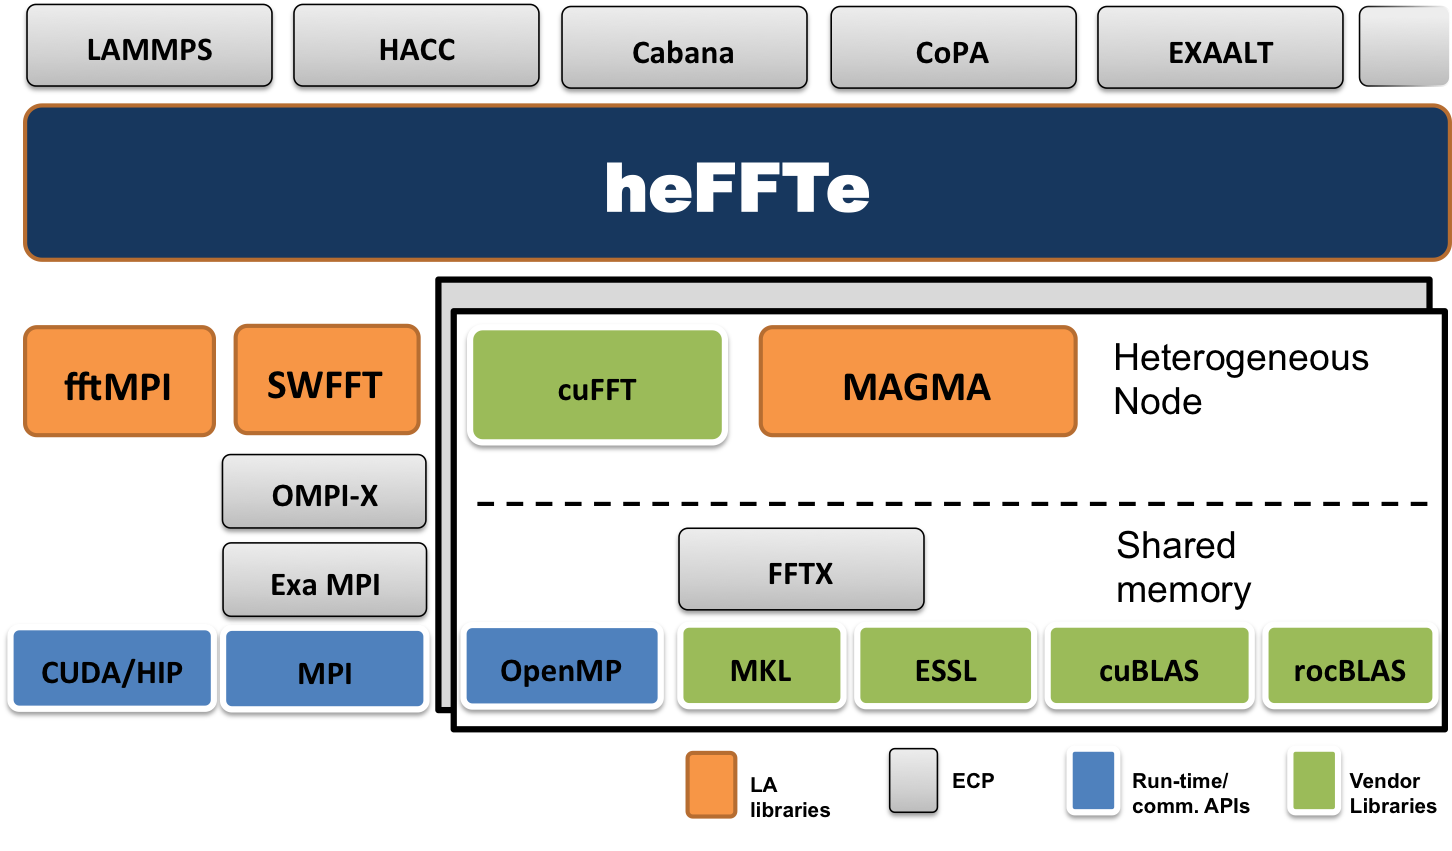
\includegraphics[width=0.42\textwidth]{projects/2.3.3-MathLibs/2.3.3.13-CLOVER/heffte}~~
    \raisebox{.4\height}{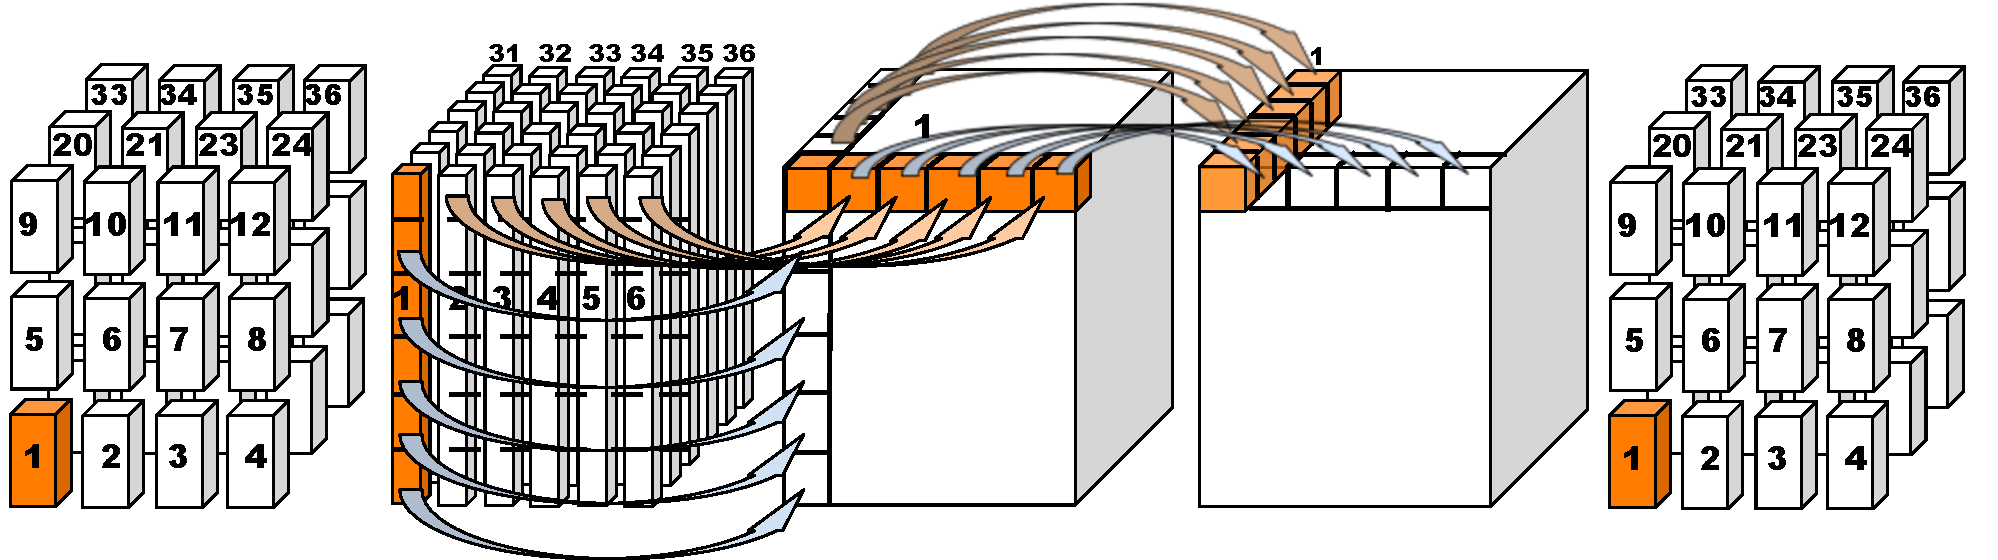
\includegraphics[width=0.56\textwidth]{projects/2.3.3-MathLibs/2.3.3.13-CLOVER/ffttransormations}}
    \caption{\label{fig:fft-ecp-pipeline}
    {\bf Left}: the heFFTe software stack. {\bf Right}: 3D FFT computational pipeline in heFFTe with:~
      1) Flexible API for application specific input and output,
         including bricks/pencils/etc.;~
      2) Efficient packing/unpacking and MPI communication
         routines;~
      3) Efficient 1D/2D FFTs on the node.}
\end{figure}

\paragraph{Key  Challenges}
\begin{enumerate}
\item
\textbf{Communication costs:}
%Today's machines have very complex memory hierarchies and thus data movement, 
%data layout translation, and communication should be the main focus of any 
%distributed FFT library that aims to improve the performance of any ECP 
%application that relies on FFT. 
Communication costs are main bottleneck 
on current systems; this includes low node bandwidth (relative to 
high compute capabilities), sub-optimal accelerator-aware MPI communications,
and encountered performance degradations in MPI implementations.

\item
\textbf{Appplication specifics:}
ECP applications that require FFT-based solvers suffer from the lack of fast 
and scalable FFTs for distributed-heterogeneous parallel systems 
as the ones projected for the upcoming exascale computing systems. Also, ECP 
applications need different application-specific versions of FFTs,
and dictate parallelism and data distributions (where is the data, how is 
distributed, what is the parallelism, etc.). This requires application
knowledge and API designs with a suitable modular high-performance 
implementation that is flexible and easy to use and integrate in ECP applications.

\item
\textbf{Performance portability:}
Performance portability across different architectures is always a challenge.
This is further exacerbated due to the many application and 
hardware-specific FFT versions needed.
\end{enumerate}

\paragraph{Solution Strategy}

\begin{enumerate}
\item
\textbf{Communications and GPU optimizations:}
FFTs are communication bound and a main focus in heFFTe is on algorithmic
design to minimize communication and efficient GPU implementations~\cite{eurompi19}.
Other strategies include the use of mixed-precision calculations~\cite{Haidar2018,tcfft18}
and data compression for reduced communications (including lossy, e.g., using ZFP compression).
\item
\textbf{Evolving design:}
heFFTe is designed to support the fftMPI and SWFFT functionalities,
which are already integrated in ECP applications. Thus, heFFTe benefits
directly these applications and provides integrated solutions. 
More functionalities and application-specific optimizations will be added 
at a second step to support other ECP applications. 
\item
\textbf{Autotuning:}
Performance portability will be addressed through use of standards (like 1D FFTs 
from vendors), portable linear algebra (LA) using MAGMA~\cite{Tomov_2010_pcsa}, 
and parameterized versions that will be tuned across architectures. We have extensive 
expertize and well proven track record in the development and use of autotuning techniques 
for important LA kernels~\cite{Nath2010,Kurzak2012gemmfermi}. 
\end{enumerate}

\paragraph{Recent Progress}
The FFT-ECP team completed implementation optimizations and features phase~\cite{thasd19}
and released the heFFTe v0.1 library~\cite{sc19}. heFFTe features very good strong 
scalability and performance that is close to 90\% of the roofline peak 
(see Figure~\ref{fig:fft-ecp-progress})~\cite{sc19,eurompi19}.


\begin{figure}[htb]
   \centering
   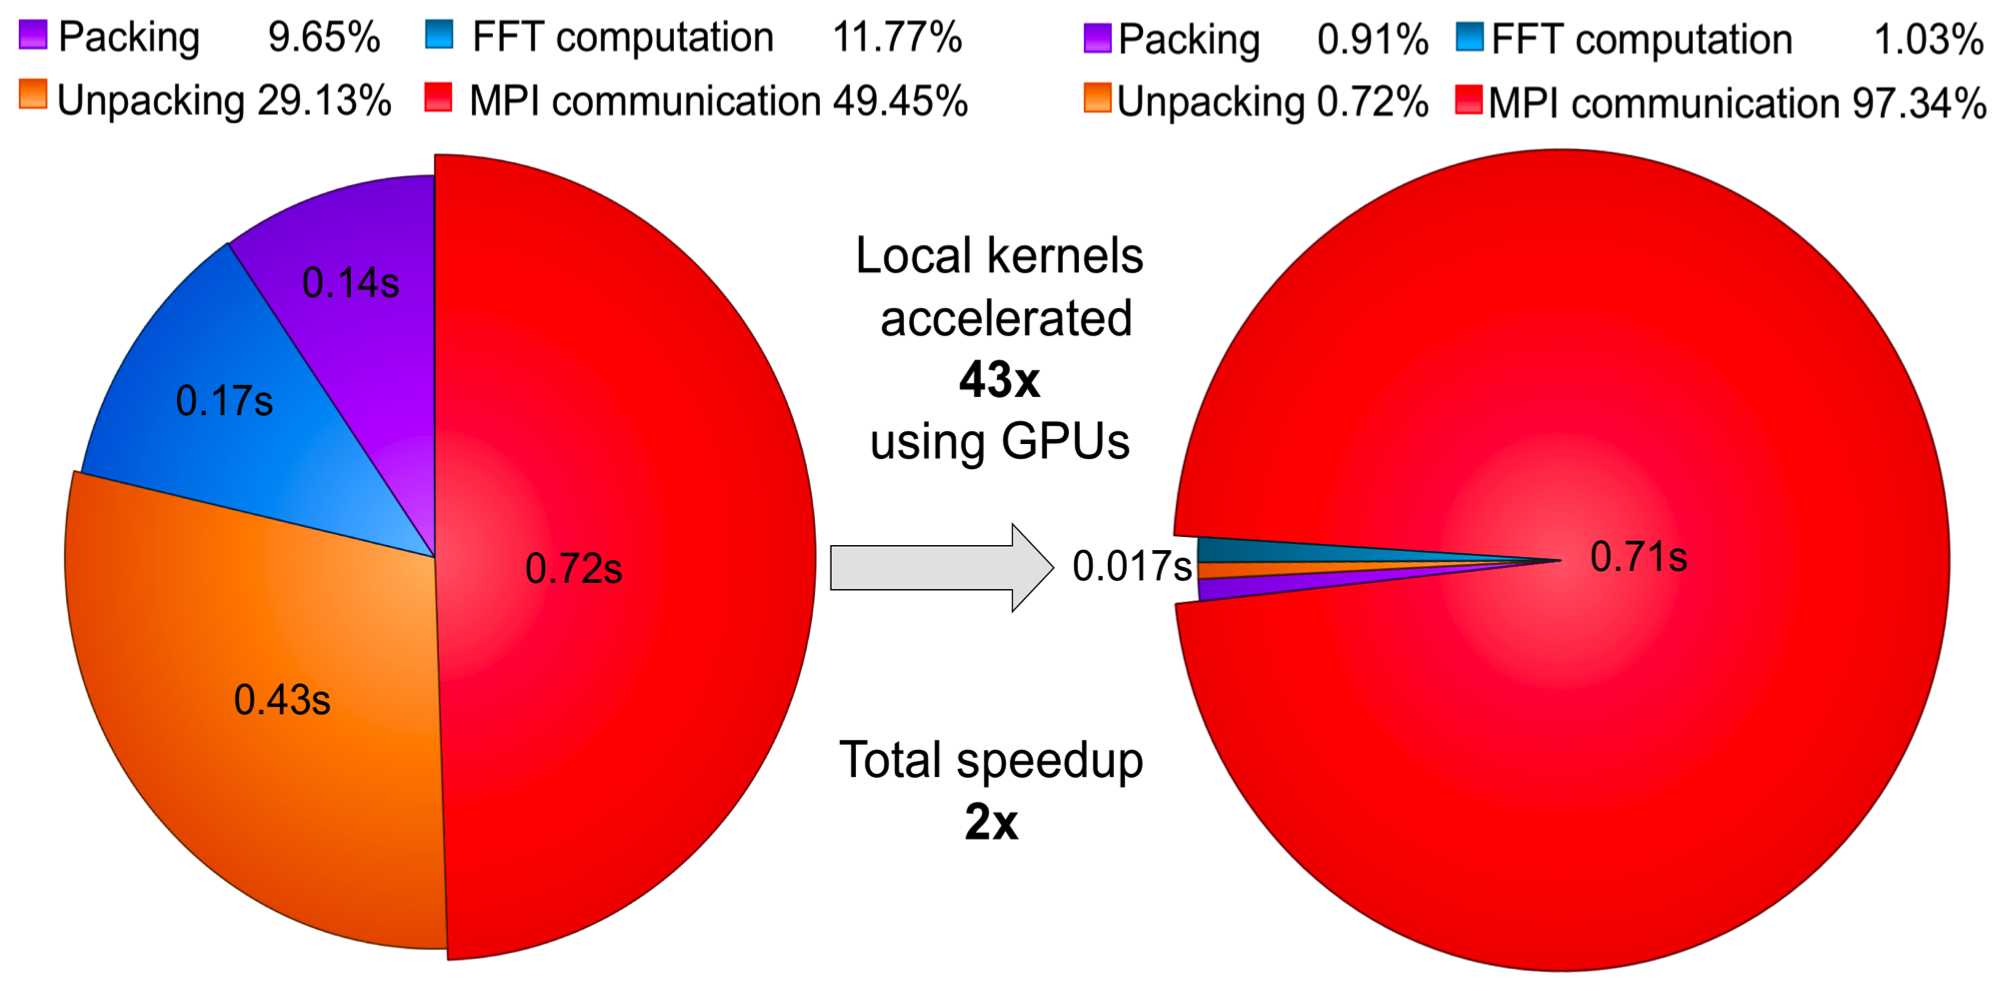
\includegraphics[width=0.55\textwidth]{projects/2.3.3-MathLibs/2.3.3.13-CLOVER/heFFTeAcceleration}~~~
   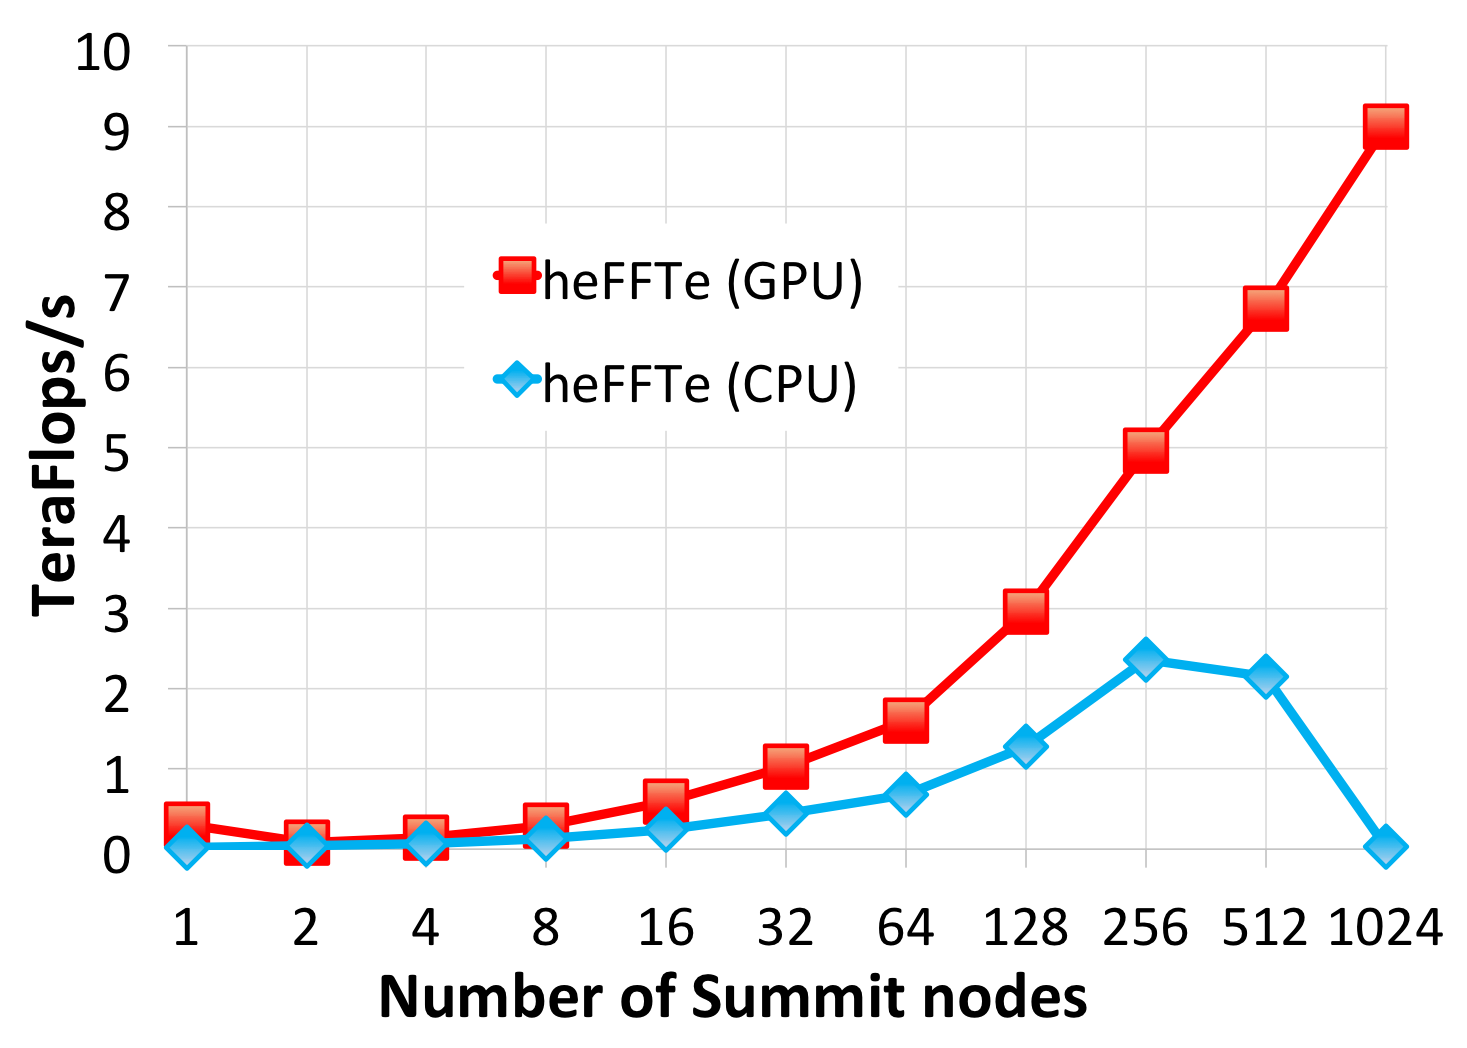
\includegraphics[width=0.38\textwidth]{projects/2.3.3-MathLibs/2.3.3.13-CLOVER/heFFTeScalability}
    \caption{\label{fig:fft-ecp-progress}
    {\bf Left}: heFFTe acceleration of $1024^3$ FFT on 4 Summit nodes.
                Note: nodal computations are accelerated $43\times$. 
    {\bf Right}: heFFTe strong scalability on $1024^3$ 
                FFT on up to 1024 nodes ($\times 6$ V100 GPUs;
                double complex arithmetic; starting and ending with bricks; 
                performance assumes $5 N^3 log_2 N^3$ flops).}
\end{figure}


\paragraph{Next Steps}
Use heFFTe in applications, generalize the APIs to fit application use,
add new APIs as needed, develop a benchmarking framework for MPI FFT 
communications, and MPI-based optimizations for Summit. 
Next step is also the development of HIP heFFTe to support AMD GPUs. 
